% !TeX root = ../main.tex

%\section{Background}

\subsection{Hidden Markov models}
\label{subsection:HMMs}

\textit{Hidden Markov models} (or HMMs) are comprised of a sequence of $T$ unobserved states $X_t$ $(t = 1, \ldots, T)$ which forms a Markov chain and an associated sequence of $T$ (possibly high-dimensional) observations $Y_t$ $(t = 1, \ldots, T)$. These observations are often referred to as ``emissions". The index $t$ often represents equi-spaced jumps in time. In the field of animal movement, the unobserved chain usually represents the latent behaviour of an animal (e.g. foraging, resting, migrating, etc.), while the observations are often a series of step lengths and turning angles for land animals and either depth or accelerometer data (or both) for marine animals. Each random variable in the unobserved chain $X_t$ can take one of $N$ possible values, and $X$ has initial distribution $\delta \in \bbR^N$ and probability transition matrix $\Gamma \in \bbR^{N \times N}$. In particular:
%
$$\delta_i = Pr(X_1 = i); \quad i = 1,\ldots,N$$
%
$$\Gamma_{ij} = Pr(X_{t+1} = j | X_t = i); \quad t = 1, \ldots, T-1; \enspace i,j = 1,\ldots,N $$
%
We assume that $\delta$ is the stationary distribution of $\Gamma$, implying that the hidden process runs infinitely before observations are recorded. Further, the distribution of each observation $Y_t$ depends only on the value of $X_t$ and none of the preceding observations or behavioral states, i.e. $p(y_t|x_1,\ldots, x_N, y_1,\ldots,y_{t-1},y_{t+1},\ldots,y_N) = p(y_t|x_t)$. In particular, we denote the distribution of $Y_t$ given that $X_t = i$ as $f^{(i)}(y_t)$. $f^{(1)},\ldots,f^{(N)}$ are described by a vector of parameters $\Theta = (\theta^{(1)},\ldots,\theta^{(N)})$ and hereafter are referred to as ``emission distributions". A visualization of the dependence structure can be seen in (fig \ref{fig:HMM}).
In order to estimate the parameters of an HMM, suppose data $y = (y_1,\ldots,y_T)$ are observed as a realization of an unknown HMM model. The probability transition matrix $\Gamma$ and parameters of the emission distributions $\Theta$ can be estimated by maximizing the likelihood of $y$, which we denote as $\calL_{\text{HMM}}(y;\Theta,\Gamma)$, with respect to $\Gamma$ and $\Theta$. In addition, $\calL_{\text{HMM}}(y;\theta,\Gamma)$ can be calculated using the well-known \textit{forward algorithm} \cite{Zucchini:2016} as follows:
%
$$\calL_{\text{HMM}}(y;\theta,\Gamma) = \delta P(y_1;\theta) \prod_{t=2}^T \Gamma P(y_t;\theta) \mathbf{1}_N$$
%
where $\mathbf{1}_N$ is an $N$-dimensional column vector of ones, and:
%
$$P(y_t;\theta) = \text{diag}(f^{(1)}(y_t),\ldots , f^{(N)}(y_t)).$$
%
To remove constraints when maximizing $\calL_{\text{HMM}}(y)$, we parameterize $\Gamma$ using $\eta \in \bbR^{N \times N}$ and the following link function \cite{Barajas:2017}:
%
$$\Gamma_{ij} = \frac{\exp(\eta_{ij})}{\sum_{j'=1}^N \exp(\eta_{i(j')})}, \qquad \eta_{ii} = 0 \quad i = 1, \ldots, N$$
%
$\eta_{ii}$ is set to zero for identifiability, and $\calL_{\text{HMM}}(y;\theta,\Gamma)$ can be maximized using any numerical optimizer.

\begin{figure}[h!]
	\centering
	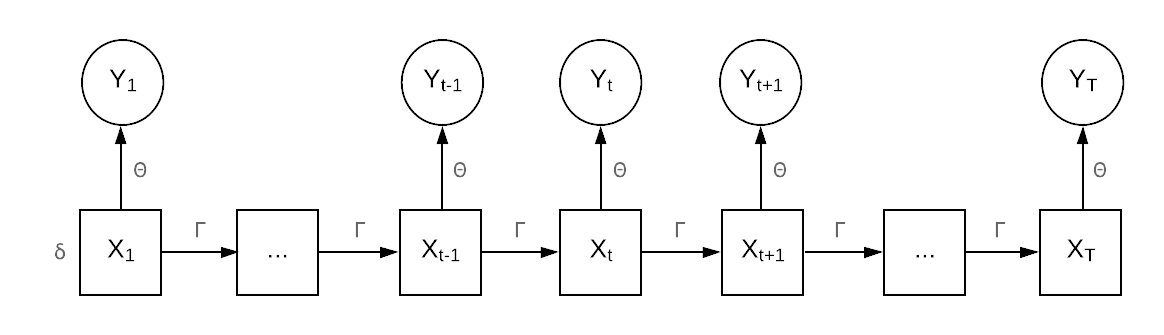
\includegraphics[width=5in]{../Plots/HMM.png}
	\caption{Graphical representation of a traditional HMM.}
	\label{fig:HMM}
\end{figure}

\subsection{Hierarchical HMMs}

Hidden Markov models are useful when inferring a single unobserved process, but biological processes often involve multiple simultaneous hidden processes which can occur and at different time scales. For example, a preliminary observation of the killer whale dive data shown in (fig \ref{fig:data}) shows that the behavior of the killer whale changes between approximately hour-long periods of predominately short, shallow dives and long, deep dives. Leos-Barajas et al. \cite{Barajas:2017} encounter a similar issue when modeling the movement of a harbor porpoise in the North Sea, and use it as a motivating example when they introduce hierarchical hidden Markov models.

\begin{figure}[h!]
	\centering
	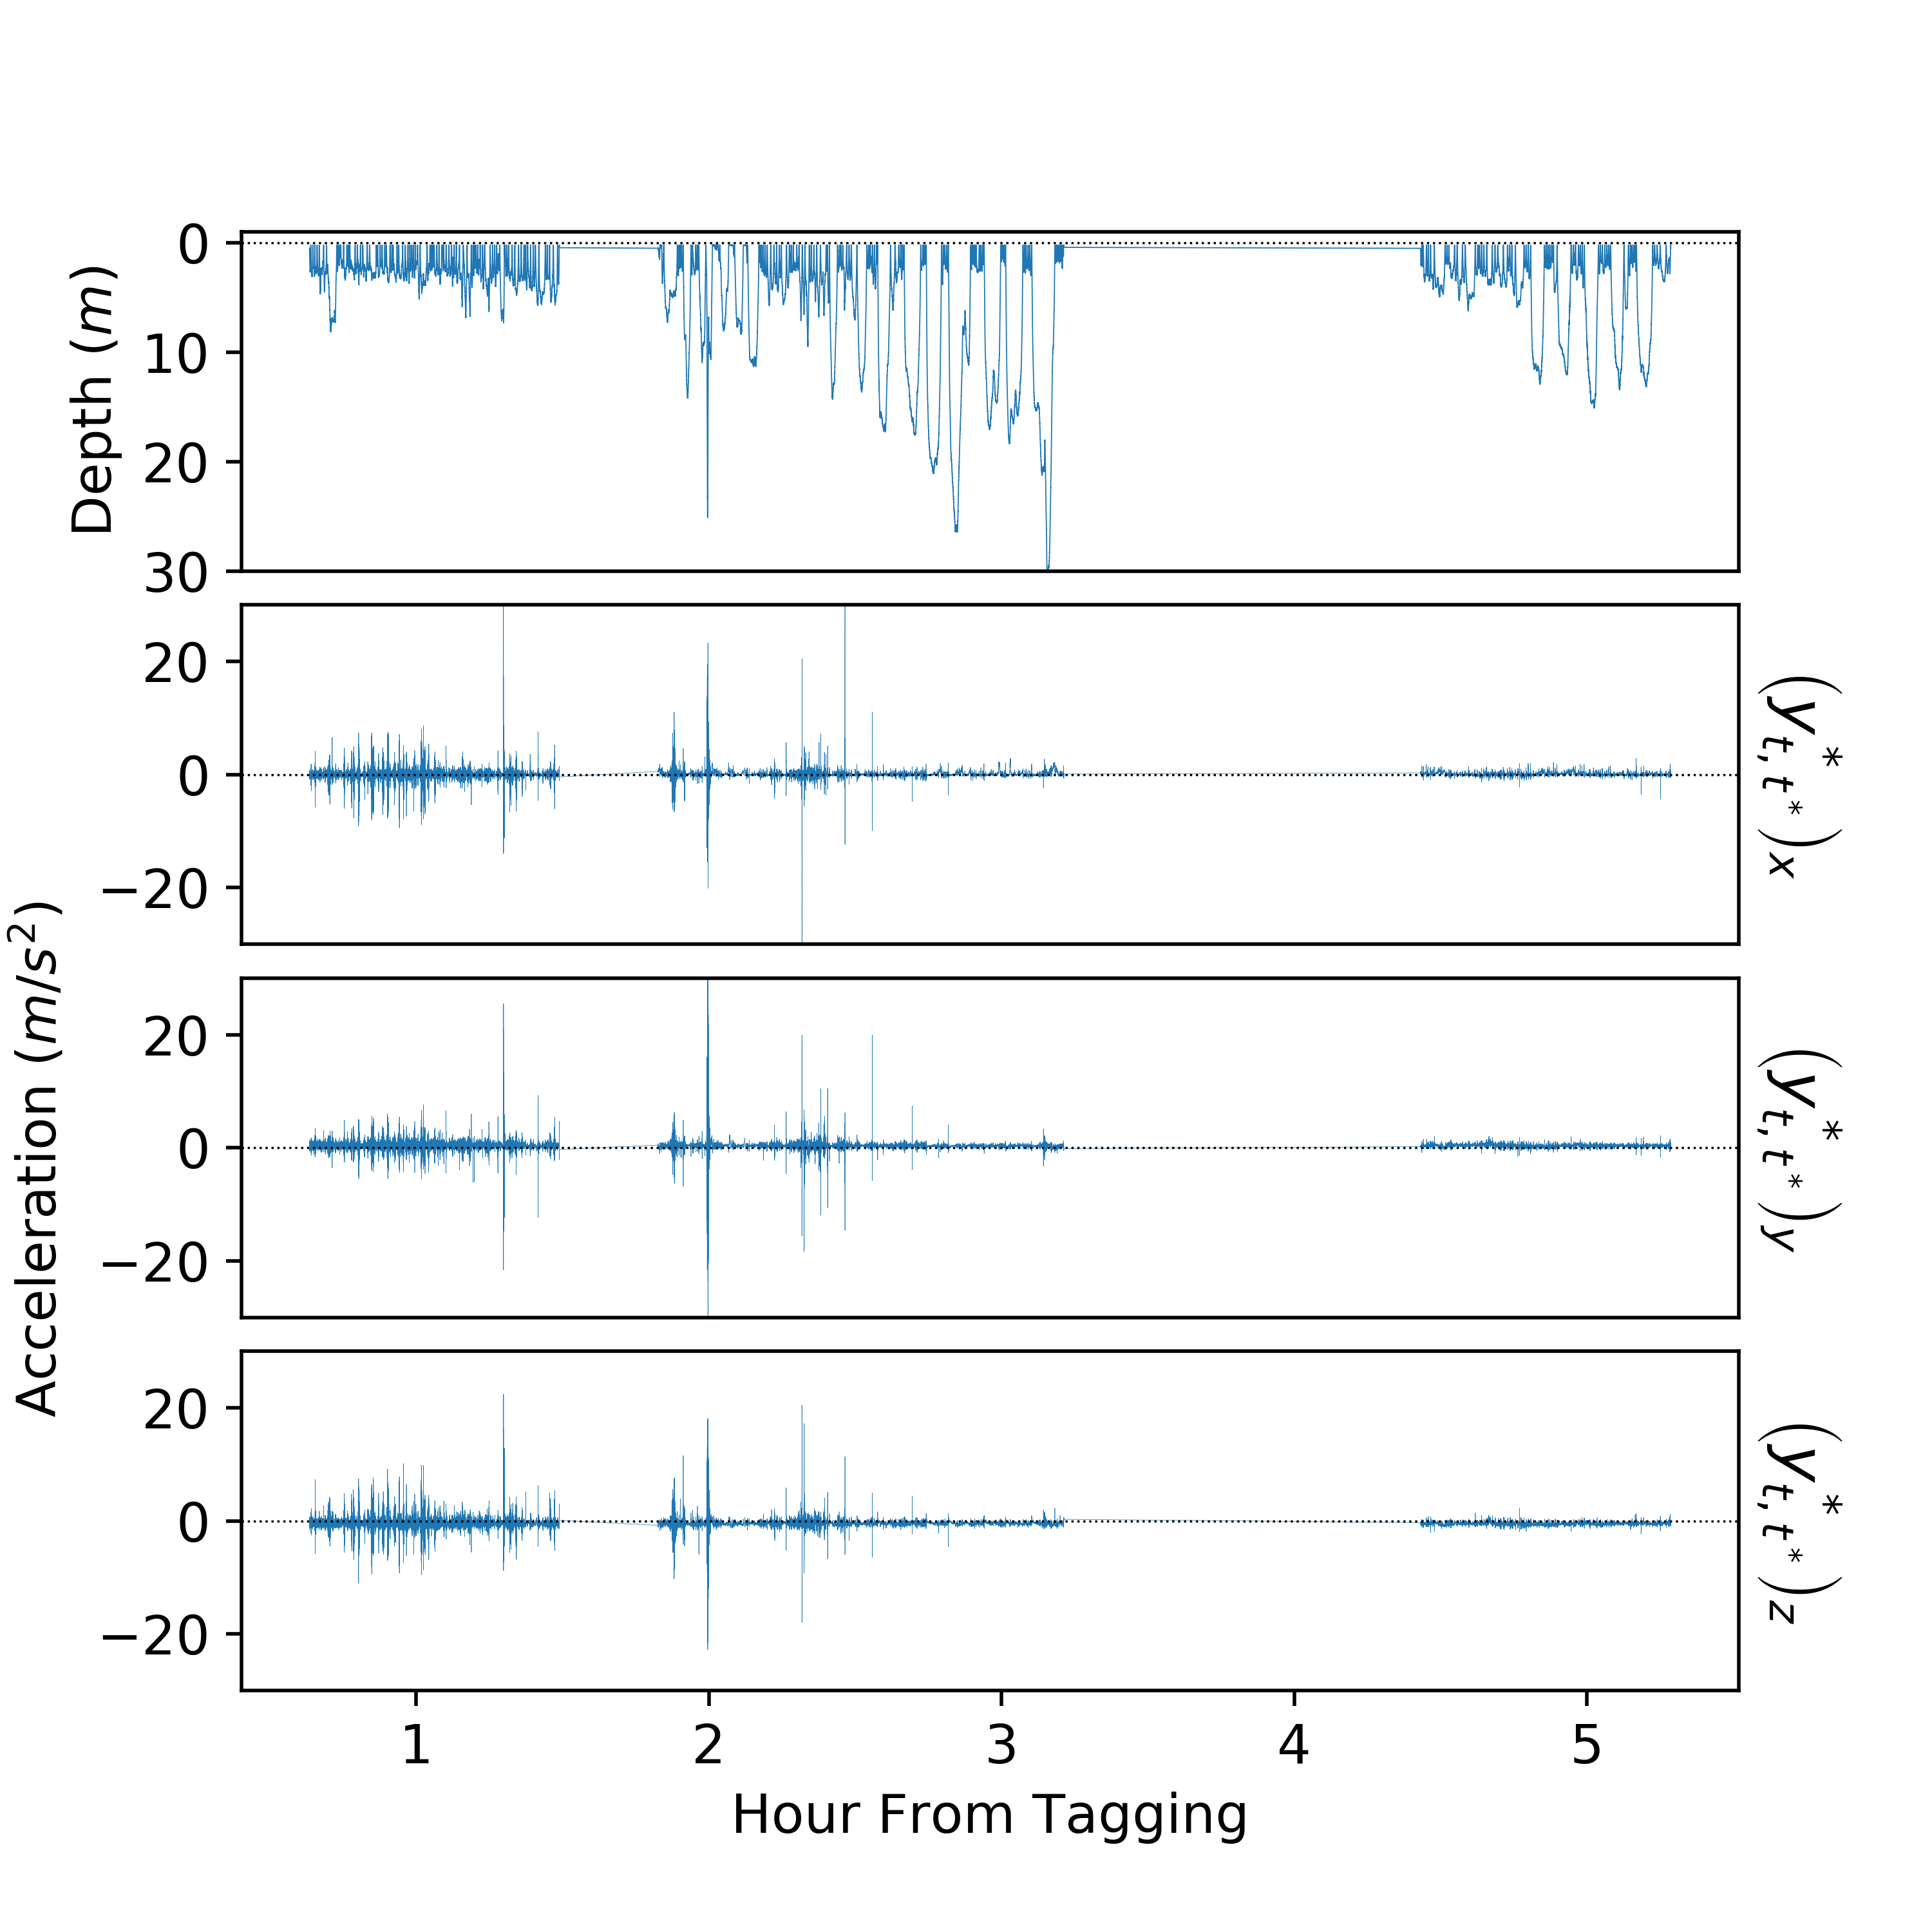
\includegraphics[width=5.5in]{../Plots/raw_data.png}
	\caption{Raw depth data of a Killer Whale off the coast of British Columbia, Canada. \textcolor{red}{I WILL REFORMAT THIS PLOT LATER.}}
	\label{fig:data}
\end{figure}

A hierarchical hidden Markov model (or HHMM) is a variation of a hidden Markov model in which $X_t$ satisfies the conditions of section \ref{subsection:HMMs}, but in addition it ``emits" yet another fine-scale hidden Markov model of length $T_t^*$. This fine-scale hidden Markov model can be either instead of \cite{Barajas:2017} or in addition to \cite{Adam:2019} a coarse-scale observation $Y_t$, which itself must satisfy the conditions from section \ref{subsection:HMMs}. The fine-scale HMM is comprised of a fine-scale Markov chain $X^*_t = (X^*_{t,1}, \ldots, X^*_{t,T^*_t})$ and fine-scale observations $Y^*_t = (Y^*_{t,1}, \ldots, Y^*_{t,T^*_t})$, each of length $T^*_t$. $X^*_t$ can take one of $N^*$ values. Note that while $N^*$ can be set to depend upon $X_t$, we assume here that it does not for simplicity in both the model presented here and the notation. Conditioned on the coarse-scale hidden state $X_t = i$, $X^*_t$ is characterized by an initial distribution $\delta^{*(i)} \in \bbR^{N^*}$ and probability transition matrix $\Gamma^{*(i)} \in \bbR^{N^* \times N^*}$:
%
$$\delta^{*(i)}_{i^*} = Pr(X^*_{t,1} = i^* | X_t = i); \quad i^* = 1,\ldots,N^*$$
%
$$\Gamma^{*(i)}_{i^*j^*} = Pr(X^*_{t,t^*+1} = j^* | X^*_{t,t^*} = i^*, X_t = i); \quad t^* = 1, \ldots, T^*_t-1; \enspace i^*,j^* = 1,\ldots,N^*$$
%
Again, although not necessary, we assume that the initial distribution $\delta^{*(i)}$ is the stationary distribution of $\Gamma^{*(i)}$. In total, there are $N$ different values that $\Gamma^{*(i)}$ and $\delta^{*(i)}$ can take- one for each possible value of the coarse-scale process $X_t$. We denote the sets of all fine-scale initial distributions and probability transition matrices as $\delta^*$ and $\Gamma^*$, respectively, where $|\delta^*| = |\Gamma^*| = N$.

Each fine-scale observation $Y^*_{t,t^*}$ depends only on the value of its corresponding fine-scale hidden state $X^*_{t,t^*}$ and coarse-scale hidden state, $X_t$. In particular, $p(y^*_{t,t^*} | y^*_{t,1}, \ldots y^*_{t,t^*-1},y^*_{t,t^*+1},\ldots,y^*_{t,T^*_t},x^*_t,x,y) = p(y^*_{t,t^*}|x^*_{t,t^*},x_t)$. We denote the distribution of $Y^*_{t,t^*}$ given that $X_t = i$ and $X^*_{t,t^*} = i^*$ as $f^{*(i,i^*)}(y^*_{t,t^*})$. Conditioned on the fact that $X_t = i$, the fine-scale distributions $f^{*(i,1)}, \ldots, f^{*(i,N^*)}$ are parameterized by an $N^*$-dimensional vector of parameters $\Theta^{*(i)} = (\theta^{*(i,1)},\ldots,\theta^{*(i,N^*)})$, where $\theta^{*(i,i^*)}$ describes the distribution $f^{*(i,i^*)}$. Depending upon the behaviour and responses being modelled, it may be desirable to force the fine-scale emission distributions to be equal across all values of $i \in \{1, \ldots, N\}: \enspace \theta^{*(1,i^*)} = \theta^{*(2,i^*)} = \ldots = \theta^{*(N,i^*)}$. A visualization of the full structure of the HHMM can be seen in (fig \ref{fig:HHMM}). 

Due to the nested structure of a hierarchical hidden Markov model, the likelihood of an HHMM is still easy to calculate using the forward algorithm. Suppose that both coarse-scale and fine scale observations ($y$ and $y^*$, respectively) are observed from an HHMM with unknown parameters. Then the likelihood of the observed data is:
%
$$\calL_{\text{HHMM}}(y,y^*;\Theta,\Theta^*,\Gamma,\Gamma^*) = \delta P(y_1,y_1^*;\Theta,\Theta^*,\Gamma^*) \prod_{t=2}^T \Gamma P(y_t,y_t^*;\Theta,\Theta^*,\Gamma^*) \mathbf{1}_N$$
%
where:
%
\begin{align*}
	P(y_t,y_t^*;\Theta,\Theta^*,\Gamma^*) = \text{diag}\Big[&f^{(1)}(y_t)\calL_{\text{HMM}}\left(y_t^*;\Theta^{*(1)},\Gamma^{*(1)}\right),\ldots, \\
	&f^{(N)}(y_t)\calL_{\text{HMM}}\left(y_t^*;\Theta^{*(N)},\Gamma^{*(N)}\right) \Big]
\end{align*}
%
Note that this formulation assumes that the coarse-scale observations at a given time $Y_t$ and the fine-scale observation time series $Y_t^*$ are independent of one another when conditioned on $X_t$. For more information on specific considerations for HHMMs such as incorporating covariates into the probability transition matrix, model selection and model checking, see Adam et al \cite{Adam:2019}.

\begin{figure}[h!]
	\centering
	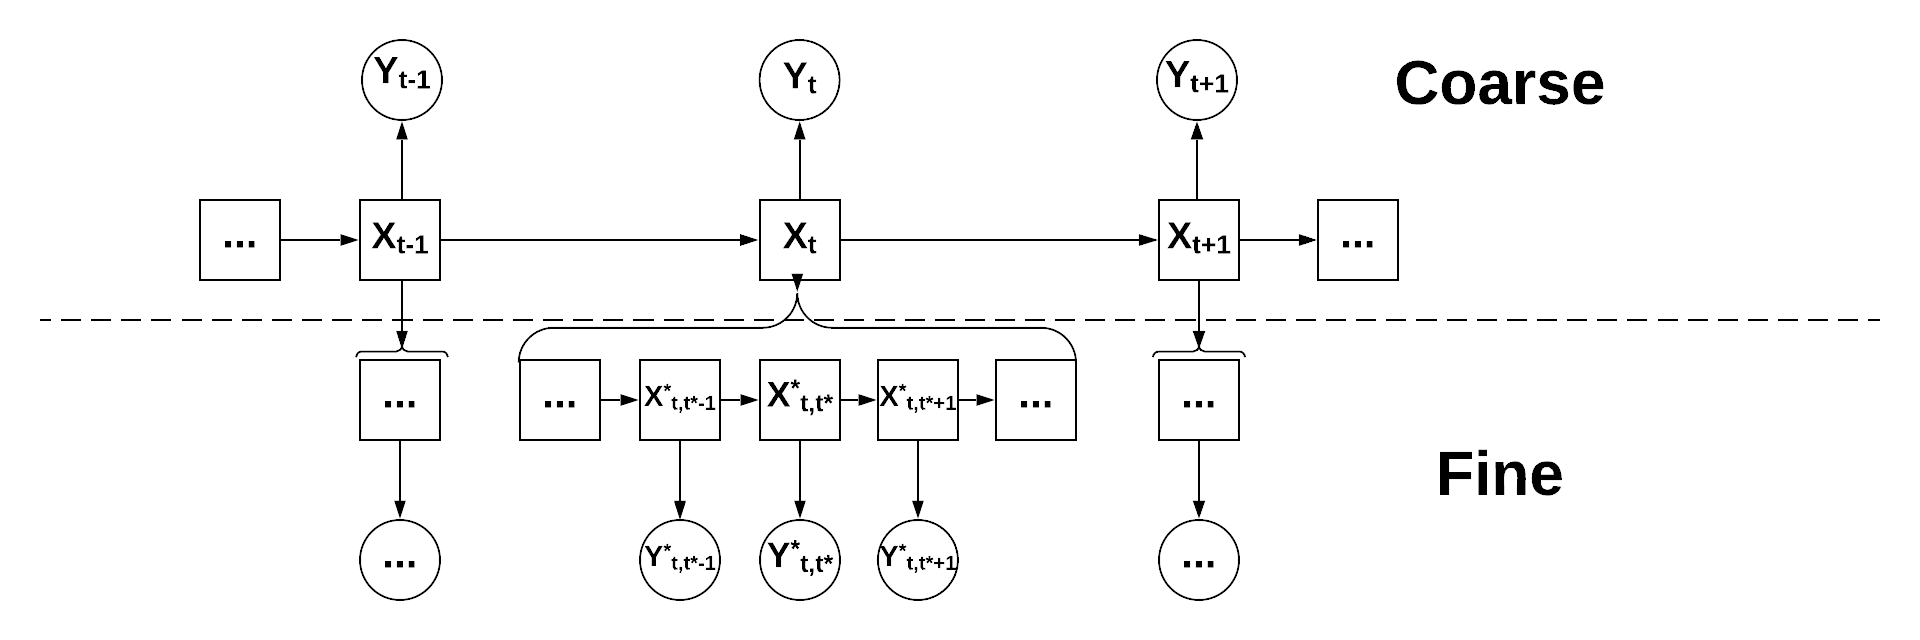
\includegraphics[width=6.5in]{../Plots/HHMM.png}
	\caption{Graphical representation of a traditional HHMM.}
	\label{fig:HHMM}
\end{figure}


\subsection{conditionally auto-regressive HMMs}

One of the key assumptions of both HMMs and HHMMs is \textit{conditional independence} between observations on both the coarse and fine scale. Namely, when given the state $X_t$, $Y_t$ is assumed to be independent from all other observations, including $Y_{t-1}$. Therefore, traditional HMMs and HHMMs can fail when the observations $Y$ exhibit significant correlation in time. Examples include fluking in marine mammals in Vancouver, BC (see the results section) and the swimming behavior of horn sharks off the coast of Southern California \cite{Adam:2019}.

One way to deal with auto-correlation in fine-scale behavioral processes is to use the CarHMM, or \textit{conditionally auto-regressive hidden Markov model}, introduced by Lawler et al \cite{Lawler:2019}. In particular, the CarHMM describes the distribution of $(Y_t|Y_{t-1}, X_t=i)$ with parameters $\theta^{(i)} = \{\mu^{(i)},\sigma^{2(i)},\phi^{(i)}\}$, where:
%
$$\mathbb{E}(Y_t|Y_{t-1} = y_{t-1},X_t=i) = \phi^{(i)}*y_{t-1} + (1-\phi^{(i)}) * \mu^{(i)}$$
$$\mathbb{V}(Y_t| X_t = i) = \sigma^{2(i)}$$
%
The CarHMM therefore explicitly models auto-correlation into the emission distributions of the HMM while maintaining the structure needed to run the forward algorithm. It also only adds one additional parameter per possible hidden state $(\phi^{(i)})$. 

The likelihood of CarHMM is still compatible with the forward algorithm, and is therefore easy to calculate:
\begin{equation}
\calL_{\text{CarHMM}}(y;\Theta,\Gamma) = \delta \prod_{t=2}^T \Gamma P(y_t;\Theta) \mathbf{1}_N
\label{CarHMM_likelihood}
\end{equation}
where:
%
$$P(y_t;\Theta) = \text{diag}\left(f^{(1)}(y_t|y_{t-1}), \ldots , f^{(N)}(y_t|y_{t-1}) \right)$$
%
and the first observation $y_1$ is assumed to be fixed as an initial value. The graphical model associated with the structure of a CarHMM is shown in figure (\ref{fig:CarHMM}).

\begin{figure}[h!]
	\centering
	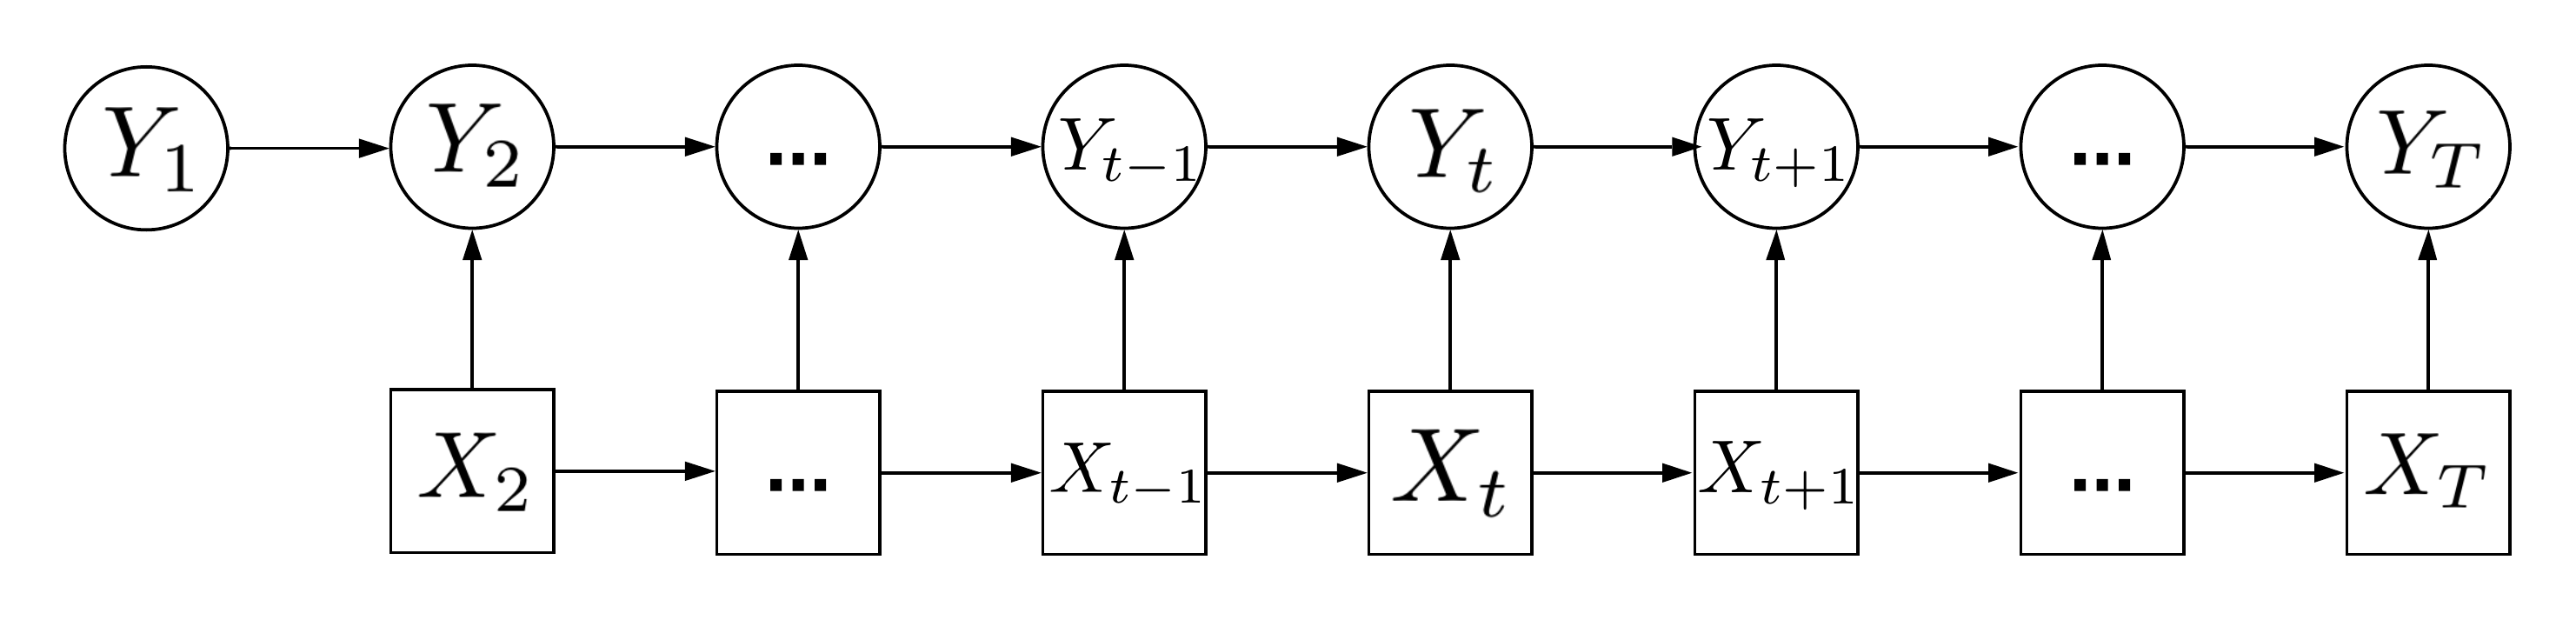
\includegraphics[width=3in]{../Plots/CarHMM.png}
	\caption{Graphical representation of a traditional CarHMM. The additional arrows representing auto-correlation between observations are shown in red for emphasis.}
	\label{fig:CarHMM}
\end{figure}


\subsection{State decoding}

Once an HMM, HHMM, or CarHMM model is fit by maximizing its respective likelihood with respect to its parameters, it is common to find the most likely sequence of hidden states $\hat X$. 

This can be done in one of two ways: first, the most likely \textit{sequence} of \text{all} hidden states can be found using a dynamic programming algorithm called the Viterbi algorithm \cite{Viterbi:1967}. Alternatively, the probability of \textit{each} coarse-level state (conditioned on the learned parameters) can be found using the \textit{forward-backward algorithm}. Both the Viterbi algorithm and the forward-backward algorithm are easy to extend to Hierarchical HMMs by recursively running the algorithm on the fine-scale HMMs after decoding the hidden states of the coarse-scale process.

While both the Viterbi algorithm and the forward-backward algorithm are used in the current ecology literature, we use the \textit{forward-backward algorithm} in this work for several reasons. First, the forward-backward algorithm is used to find the \textit{psuedoresiduals} of a given model, which are an important tool for model validation. In addition, the forward-backward algorithm can be implemented recursively to find the probability of the fine-level states $X^*_{t^*,t}$ exactly by marginalizing out $X_t$:
%
$$P(X^*_{t^*,t} = i^*) = \sum_{i=1}^N P(X_t = i)P(X^*_{t^*,t} = i^* | X_t = i)$$
%
where $P(X_t = i)$ can be found using the forward-backward algorithm on the coarse-level Markov chain and $P(X^*_{t^*,t} = i^* | X_t = i)$ can be found by running the forward-backward algorithm on the fine-scale HMM.